\subsection{\label{sec:calib.dc}Drift Chamber Calibration and Resolution}

\subsubsection{\label{sec:DC.TOF.res}Drift Chamber and TOF smearing parameters in \prog{gpp}}

Tracking in the Drift Chamber of a \abbr{CLAS} Sector is performed using the six superlayers of the \abbr{DC}. A good measure of the the quality of tracking are the \abbr{DC} residuals for each superlayer. After a track is identified using the hit elements in the \abbr{DC} superlayer, It's \abbr{DC} residual is calculated using the TBLA bank as follows:

\begin{verbatim}
fabs(TBLA->tbla[i].fitdoca) - fabs(TBLA->tbla[i].calcdoca)
\end{verbatim}

The values of the DC residuals in the CLAS data are empirically found to be a good fit to a convolution of 2 gaussians - a narrow gaussian and a broad gaussian. During DC calibrations efforts were made to minimise this residual to have maximum reconstruction efficiency. The mean and width of the residuals as a function of superlayer and run number are shown in Figs.~\ref{fig:calib.dc.residuals.mean} and \ref{fig:calib.dc.residuals.wid} respectively.


\begin{figure}\begin{center}
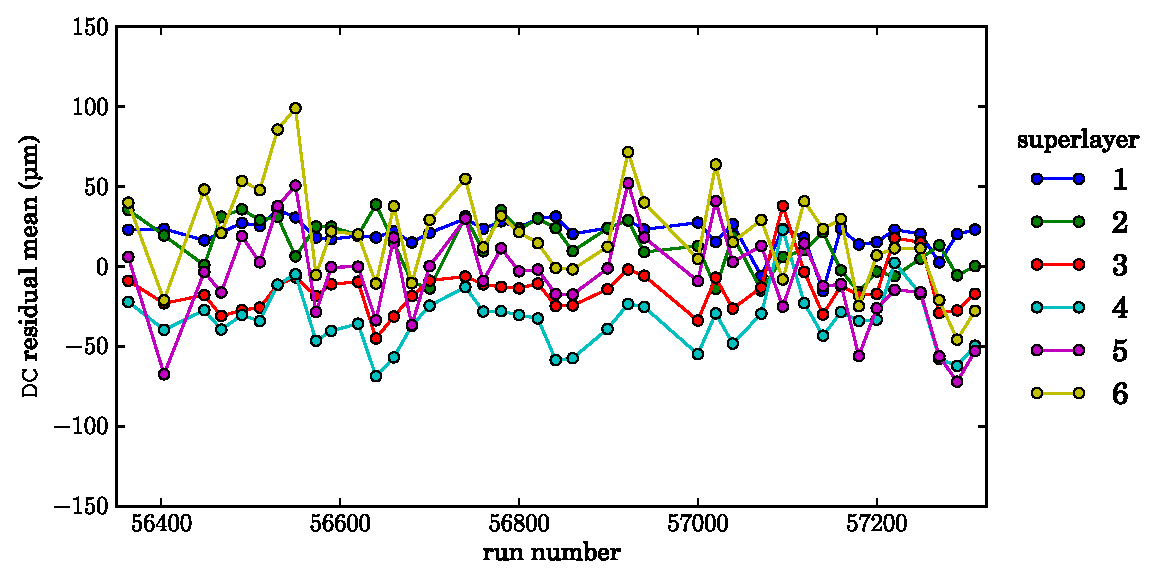
\includegraphics[width=0.6\textwidth]{figures/calib/dc/dc_resid_mean.eps}
\caption[DC Residuals (Mean)]{\label{fig:calib.dc.residuals.mean}Mean of residuals for the drift chambers by superlayer and by run.}
\end{center}\end{figure}

\begin{figure}\begin{center}
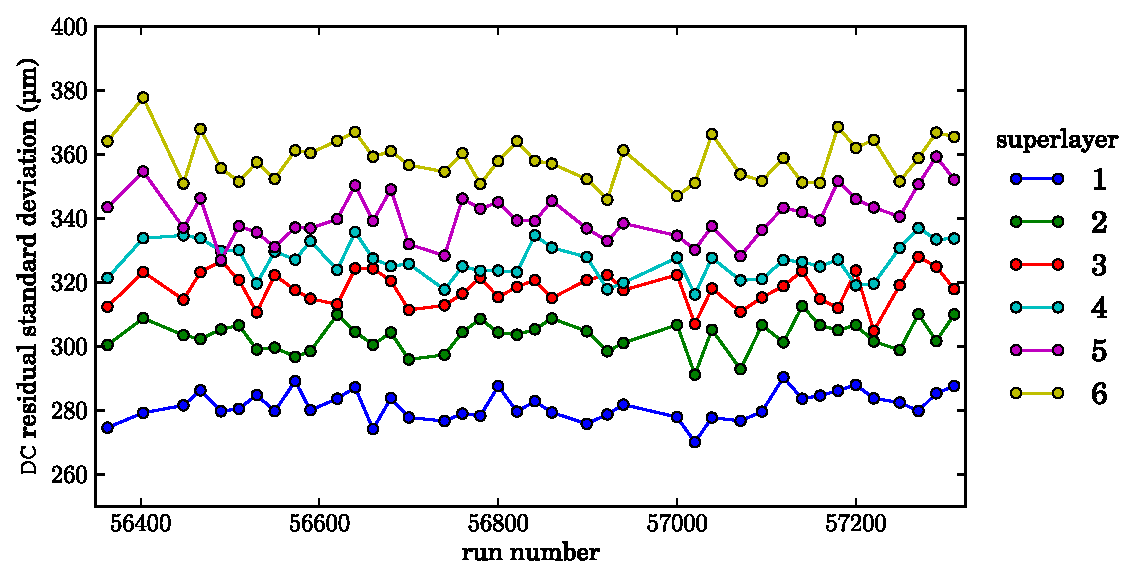
\includegraphics[width=0.6\textwidth]{figures/calib/dc/dc_resid_sigma.eps}
\caption[DC Residuals (Width)]{\label{fig:calib.dc.residuals.wid}Gaussian width of residuals for the drift chambers by superlayer and by run.}
\end{center}\end{figure}

\FloatBarrier

\subsubsection{\label{sec:calib.dc.eff}Drift Chamber Wire Efficiency}

\FloatBarrier
